\documentclass[a4paper, 12pt]{article}

\usepackage{hyperref}
\usepackage[warn]{mathtext}
\usepackage[utf8]{inputenc}
\usepackage[T2A]{fontenc}
\usepackage[english,russian]{babel}
\usepackage{multirow}
\usepackage{amsmath,amsfonts,amssymb,amsthm,mathtools}
\usepackage{indentfirst}
\DeclareSymbolFont{T2Aletters}{T2A}{cmr}{m}{it}
\usepackage{ gensymb }
\mathtoolsset{showonlyrefs=true}
\usepackage{euscript}
\usepackage{mathrsfs}
\usepackage[left=2cm,right=2cm,top=2cm,bottom=2cm]{geometry}
\usepackage{graphicx}
\usepackage{wrapfig}
\usepackage[rgb]{xcolor}
\hypersetup{
colorlinks=true,
urlcolor=blue
}


\title{Лабораторная работа}
\author{Гисич Арсений Б03-102}
\date{2022}

\begin{document}

	\begin{center}
		{\large МОСКОВСКИЙ ФИЗИКО-ТЕХНИЧЕСКИЙ ИНСТИТУТ (НАЦИОНАЛЬНЫЙ ИССЛЕДОВАТЕЛЬСКИЙ УНИВЕРСИТЕТ)}
	\end{center}
	\vspace{5 cm}
	{\Large
		\begin{center}
			{\bf Лабораторная работа 3.3.4}\\[0.2 cm]
			Эффект Холла в полупроводниках
		\end{center}
	}
	\vspace{4 cm}
	\begin{flushright}
		{\Large Выполнил: \\
			\vspace{0.2 cm}
			Гисич Арсений \\
			\vspace{0.2 cm}
			Б03-102 \\}
	\end{flushright}
	\vspace{9 cm}
	\begin{center}
		Долгопрудный\\[0.1 cm]
		2022
	\end{center}
\thispagestyle{empty}

\section{Аннотация}

В данной работе исследовалась зависимость ЭДС Холла от величины магнитного поля при различных значениях тока через образец для определения константы Холла. Также был определён знак носителей заряда и проводимость материала образца.

\section{Теоретические сведения}

Суть эффекта Холла состоит в следующем. Пусть через однородную пластину металла вдоль оси $x$ течет ток $I$ (рис.~\ref{ris1}).
	
\begin{wrapfigure}{l}{0.6\textwidth}
	\vspace{-20pt}
	\begin{center}
		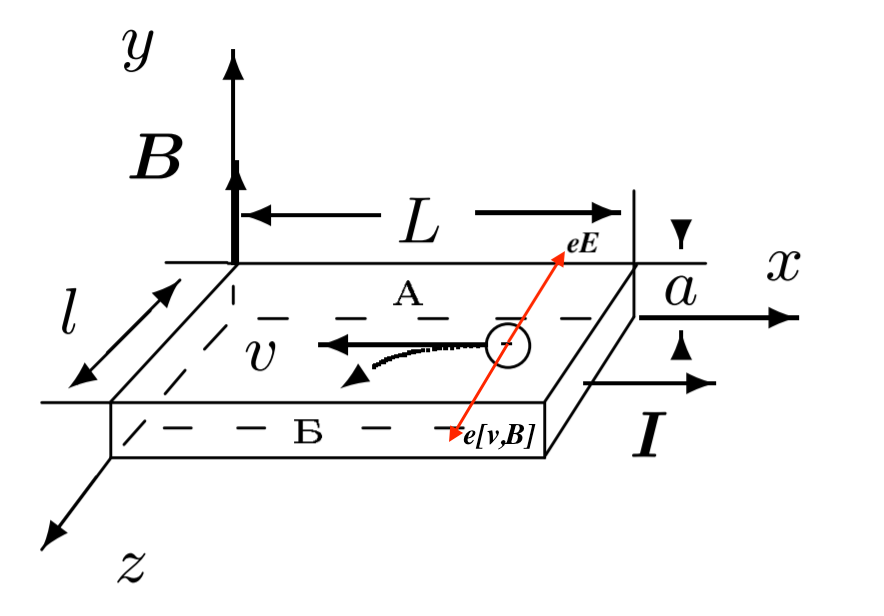
\includegraphics[width=0.7\linewidth]{1.png}
		\label{ris1}
	\end{center}
	\vspace{-20pt}
	\caption{Образец с током в магнитном поле}
\end{wrapfigure}

	Если эту пластину поместить в магнитное поле, направленное по оси y, то между гранями А и Б появляется разность потенциалов. 
	
	В самом деле, на электрон (для простоты рассматриваем один тип носителей), движущийся со средней скоростью $\langle \vec{v} \rangle$ в электромагнитном поле, действует сила Лоренца:
	
	$$\vec{F}_{л} = -e\vec{E}-e \langle \vec{v} \rangle \times \vec{B},$$
	
	где $e$ --- абсолютный заряд электрона, $\vec{E}$ --- напряженность электрического поля, $\vec{B}$ --- индукция магнитного поля.
	
	В проекции на ось $z$ получаем
	
	$$ F_{B}=e | \langle {v_{x}} \rangle | B.$$
	
	Под действием этой силы электроны отклоняются к грани Б, заряжая ее отрицательно. На грани А накапливаются нескомпенсированные положительные заряды. Это приводит к возникновению электрического поля $E_{z}$, направленного от А к Б, которое действует на электроны с силой $F_{E}=eE_{z}$. В установившемся режиме $F_{E}=F_{B}$, поэтому накопление электрических зарядов на боковых гранях пластины прекращается. Отсюда
	
	$$ E_{z}=| \langle {v_{x}} \rangle | B.$$
	
	С этим полем связана разность потенциалов $$U_{AБ}=E_{z}l=| \langle {v_{x}} \rangle | Bl.$$
	
	В этом и состоит эффект Холла.
	
	\
	
	Замечая, что сила тока
	
	$$ I=ne| \langle {v_{x}} \rangle |la,$$
	
	найдем ЭДС Холла:
	
\begin{equation}\label{Rx}
	\mathscr{E}_{X}=U_{AБ}=\dfrac{IB}{nea}=R_{X}\dfrac{IB}{a}.
\end{equation}
	
	Константа $R_{X}=\dfrac{1}{ne}$ называется постоянной Холла.
	
	В полупроводниках, когда вклад в проводимость обусловлен и электронами и дырками, выражение для постоянной Холла имеет более сложный вид:
	
	$$R_{X}=\dfrac{nb^{2}_{e}-pb^{2}_{p}}{e(nb_{e}+pb_{p})^{2}},$$
	
	где $n$ и $p$ --- концентрации электронов и дырок; $b_{e}$, $b_{p}$ --- их подвижности.

\section{Методика измерений}

Схема экспериментальной установки показана на рис.~\ref{ris2}.
	
\begin{figure}[h!]
\begin{center}
    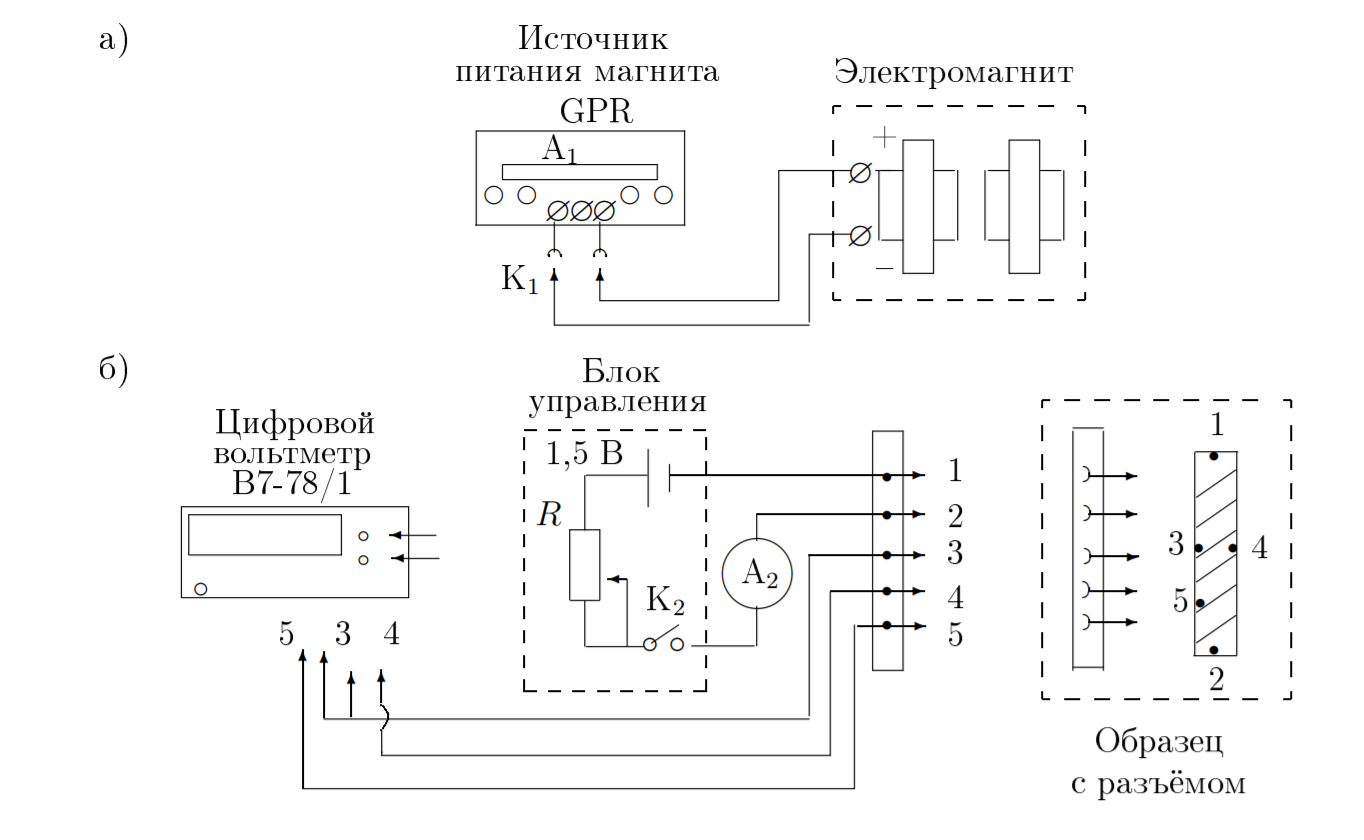
\includegraphics[width=\linewidth]{2.png}
\end{center}
\caption{Схема установки для исследования эффекта Холла в полупроводниках}
\label{ris2}
\end{figure}
  
  	В зазоре электромагнита (рис.~\ref{ris2}a) создаётся постоянное магнитное поле, величину которого можно менять с помощью регуляторов источника питания. Ток измеряется амперметром источника питания $A_{1}$. Разъем $K_{1}$ позволяет менять направление тока в обмотках электромагнита.
  
  	Образец из легированного германия, смонтированный в специальном держателе (рис.~\ref{ris2}б), подключается к батарее. При замыкании ключа $K_{2}$ вдоль длинной стороны образца течет ток, величина которого регулируется реостатом $R$ и измеряется миллиамперметром $А_{2}$.
  	
  	В образце с током, помещённом в зазор электромагнита, между контактами 3 и 4 возникает разность потенциалов $U_{34}$, которая измеряется с помощью цифрового вольтметра.
  	
  	Контакты 3 и 4 вследствие неточности подпайки не всегда лежат на одной
  	эквипотенциали, и тогда напряжение между ними связано не только с эффектом
  	Холла, но и с омическим падением напряжения, вызванным протеканием основного тока через образец.
  	
  	Измеряемая разность потенциалов при одном направлении
  	магнитного поля равна сумме ЭДС Холла и омического падения напряжения, а
  	при другом  их разности. В этом случае ЭДС Холла $\mathscr{E}_{X}$ может быть определена как половина алгебраической разности показаний вольтметра, полученных для
  	двух противоположных направлений магнитного поля в зазоре.
  	
  	Можно исключить влияние омического падения напряжения иначе, если при каждом токе через образец измерять напряжение между точками 3 и 4 в отсутствие магнитного поля. При фиксированном токе через образец это дополнительное к ЭДС Холла напряжение $U_{0}$ остается неизменным. От него следует (с учетом
  	знака) отсчитывать величину ЭДС Холла: 
  	
  	$$\mathscr{E}_{X} = U_{34} - U_{0}.$$
  	
  	При таком способе измерения нет необходимости проводить повторные измерения с противоположным направлением магнитного поля.
  	
  	
  	По знаку $\mathscr{E}_{X}$ можно определить характер проводимости --- электронный или дырочный. Для этого необходимо знать направление тока в образце и направление
  	магнитного поля.
  	
  	Измерив ток $I$ в образце и напряжение $U_{35}$ между контактами 3 и 5 в отсутствие магнитного поля, можно, зная параметры образца, рассчитать проводимость материала образца по формуле:
  	
  \begin{equation}\label{sigma}
  	\sigma=\dfrac{IL_{35}}{U_{35}ah},
  \end{equation}
  	
где $L_{35}$ --- расстояние между контактами 3 и 5, $a$ --- ширина образца, $h$ --- его толщина.
  	
\section{Используемое оборудование}

\begin{enumerate}
    \item электромагнит с регулируемым источником питания;
    \item вольтметр;
    \item амперметр;
    \item миллиамперметр;
    \item милливеберметр или миллитесламетр;
    \item источник питания;
    \item образцы легированного германия;
\end{enumerate}

\section{Результаты измерений и обработка данных}

Параметры образца:
\begin{description}
\item{} $a = 2,2~мм$
\item{} $L = 6,0~мм$
\item{} $l = 7~мм$
\end{description}

Результаты измерения калибровочной зависимости поля $B$ от тока в электромагните $I_М$ представлены в таб.~\ref{tab1}. Калибровочный график зависимости представлен на рис.~\ref{plot1}.

\begin{table}[h!]
\begin{center}
\begin{tabular}{|c|c|c|c|}
\hline
$I_М, А$ & $\delta_{I_М}, А$ & $B, мТл$ & $\delta_B, мТл$ \\ \hline
0,000 & 0,020  & 17,7   & 1,9     \\ \hline
0,210 & 0,021  & 224,8  & 12,2    \\ \hline
0,500 & 0,023  & 521,8  & 27,1    \\ \hline
0,810 & 0,024  & 802,7  & 41,1    \\ \hline
1,020 & 0,025  & 929,4  & 47,5    \\ \hline
1,220 & 0,026  & 1016,2 & 51,8    \\ \hline
1,420 & 0,027  & 1072,1 & 54,6    \\ \hline
\end{tabular}
\end{center}
\caption{Калибровочная зависимость $B(I_М)$}
\label{tab1}
\end{table}

\begin{figure}[h!]
\begin{center}
    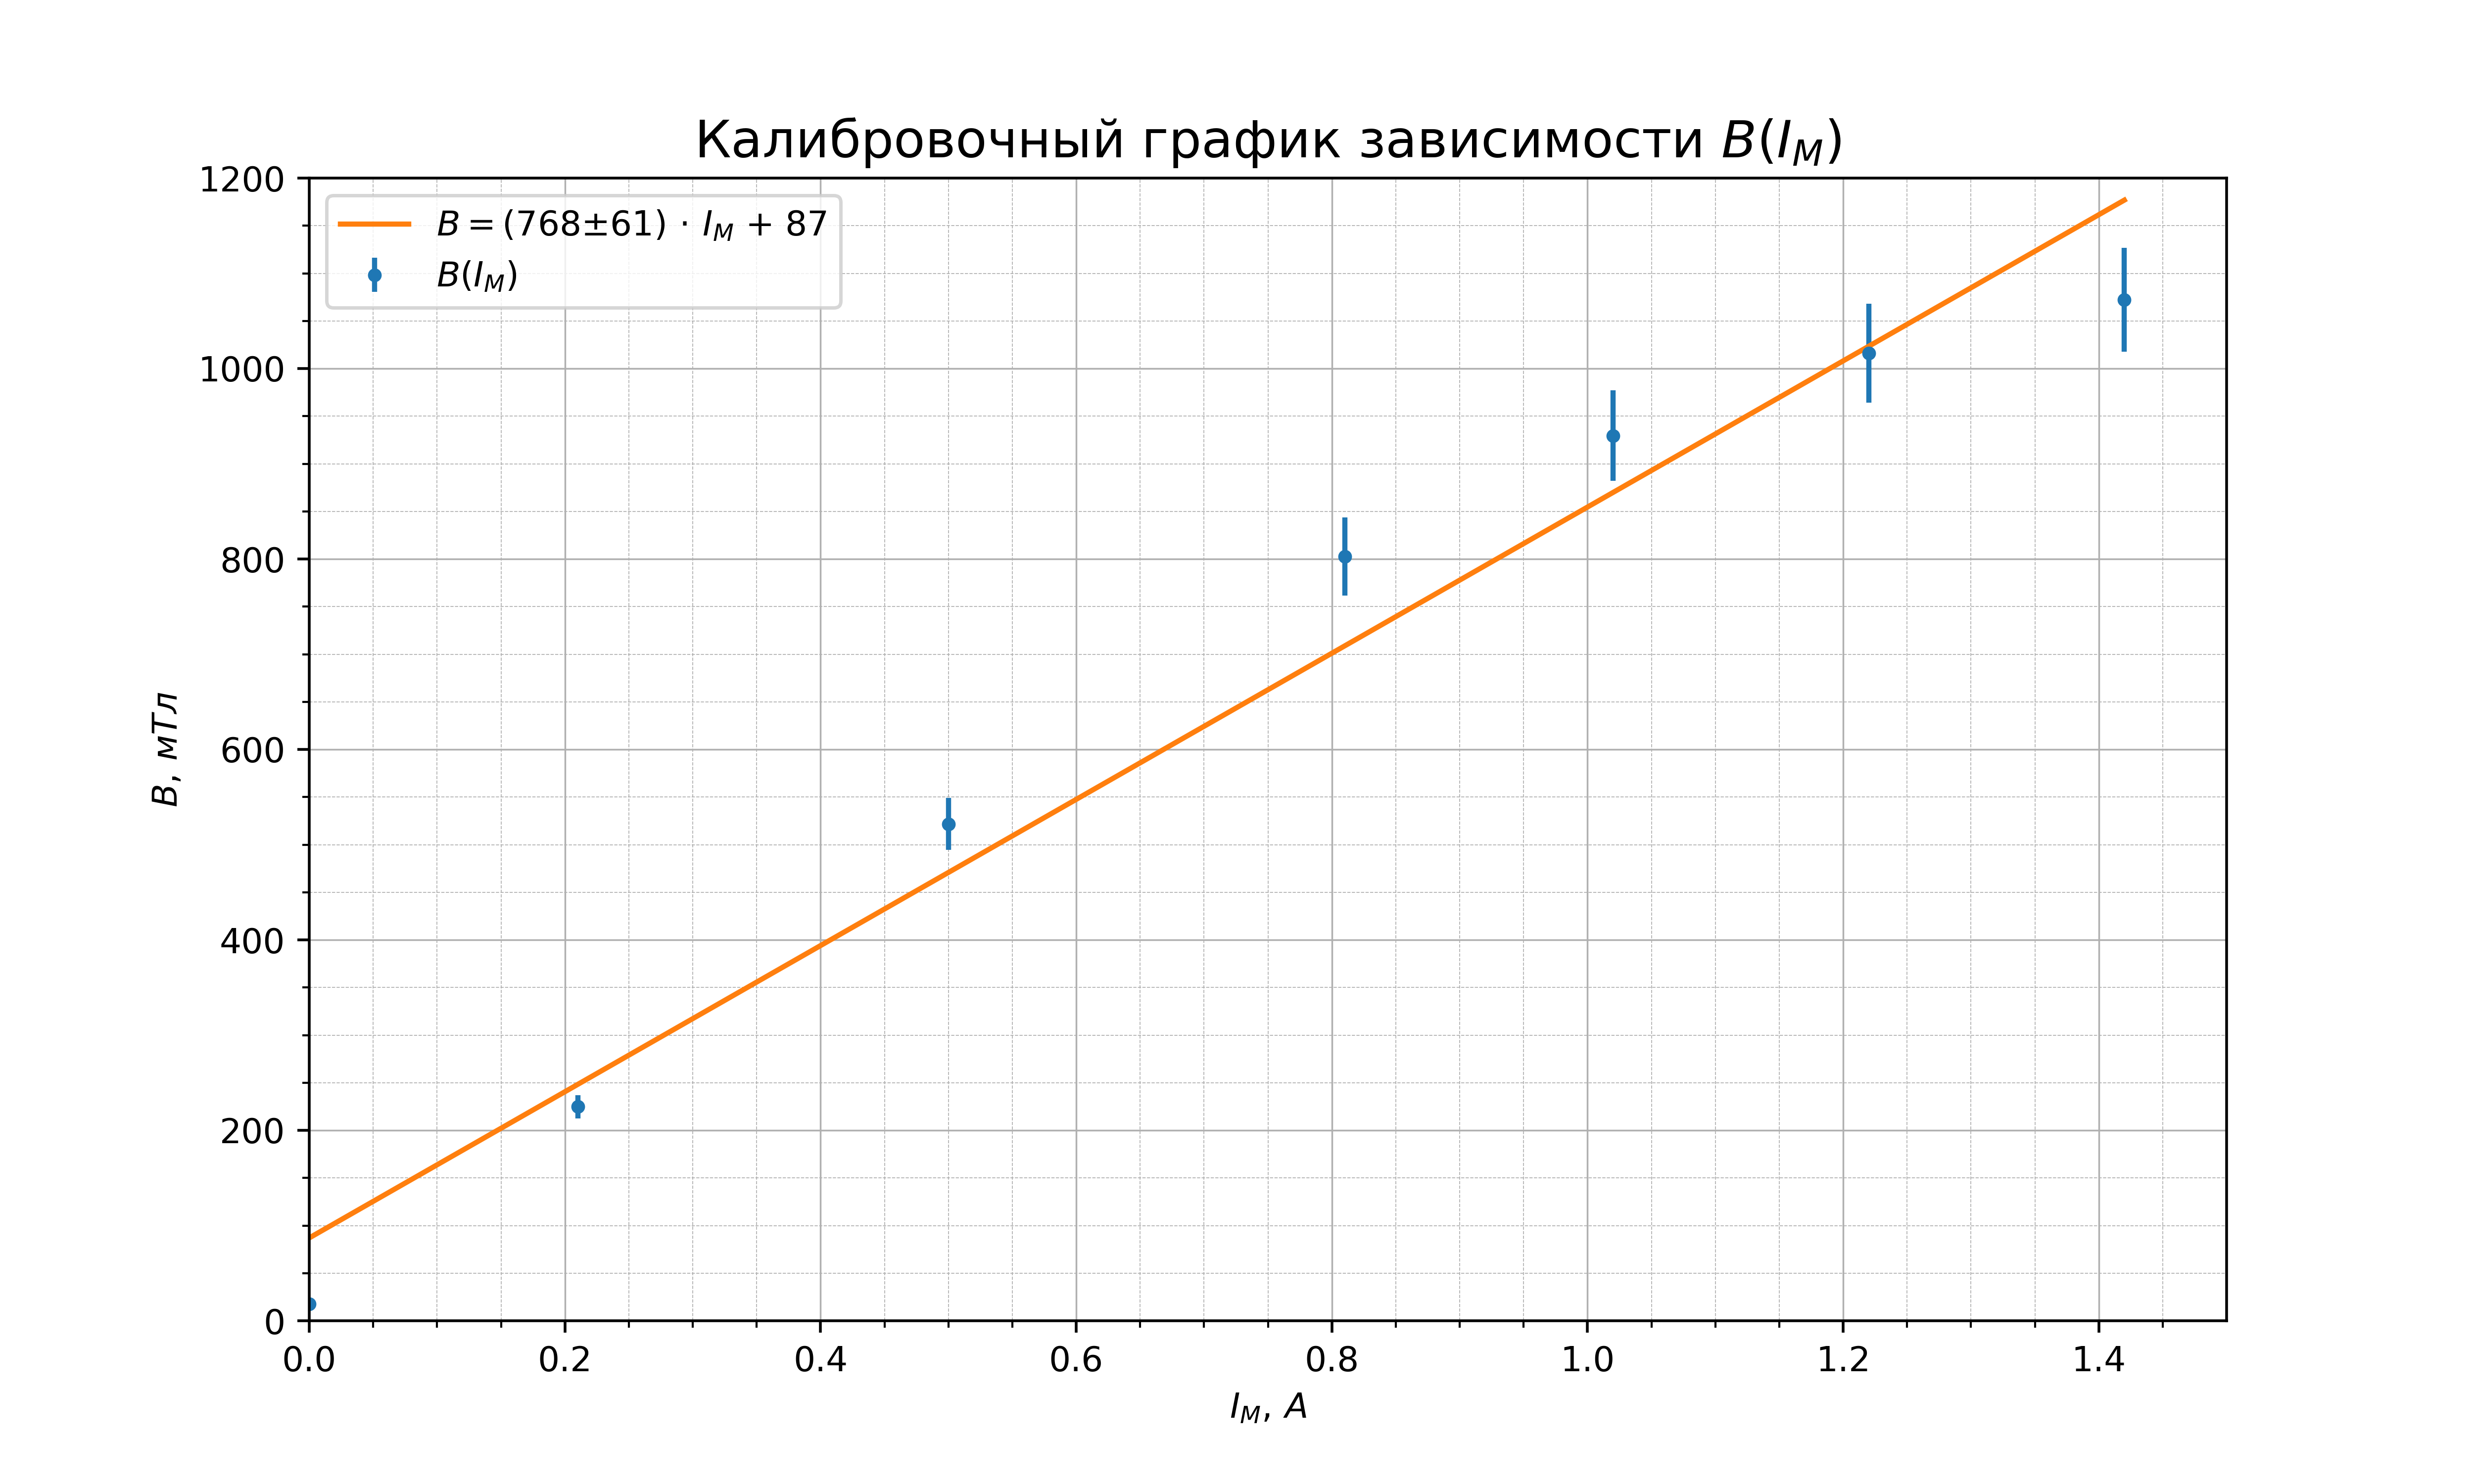
\includegraphics[scale=0.7]{3.3.4_1.png}
\end{center}
\caption{Калибровочный график}
\label{plot1}
\end{figure}

\newpage

Результаты измерений разности потенциалов $U_{34}$ между точками 3 и 4 в зависимости от поля $B$ при различных значениях тока через образец $I$ и полученные значения ЭДС Холла $U_{\perp}$ представлены в таб.~\ref{tab2}--\ref{tab9}.

\begin{table}[h!]
\begin{center}
\begin{tabular}{|c|c|c|c|c|c|}
\hline
$I_М, A$  & $\delta_{I_М}, А$ & $U_{34}, мВ$ & $U_{\perp}, мB$ & $\delta_{U_{\perp}}, мВ$ & $U_0, мВ$                     \\ \hline
0,240 & 0,021 & -0,030  & 0,030    & 0,001  & \multirow{6}{*}{-0,06} \\ \cline{1-5}
0,500 & 0,023 & 0,001   & 0,061    & 0,001  &                        \\ \cline{1-5}
0,750 & 0,024 & 0,026   & 0,086    & 0,001  &                        \\ \cline{1-5}
1,030 & 0,025 & 0,045   & 0,105    & 0,001  &                        \\ \cline{1-5}
1,230 & 0,026 & 0,054   & 0,114    & 0,001  &                        \\ \cline{1-5}
1,400 & 0,027 & 0,059   & 0,119    & 0,001  &                        \\ \hline
\end{tabular}
\end{center}
\caption{Результаты измерения ЭДС Холла при $I = 0,3~мА$}
\label{tab2}
\end{table}

\begin{table}[h!]
\begin{center}
\begin{tabular}{|c|c|c|c|c|c|}
\hline
$I_М, A$  & $\delta_{I_М}, А$ & $U_{34}, мВ$ & $U_{\perp}, мB$ & $\delta_{U_{\perp}}, мВ$ & $U_0, мВ$                     \\ \hline
0,250 & 0,021 & -0,039  & 0,042    & 0,001  & \multirow{6}{*}{-0,081} \\ \cline{1-5}
0,510 & 0,023 & 0,003   & 0,084    & 0,001  &                         \\ \cline{1-5}
0,750 & 0,024 & 0,035   & 0,116    & 0,001  &                         \\ \cline{1-5}
1,030 & 0,025 & 0,059   & 0,140    & 0,001  &                         \\ \cline{1-5}
1,240 & 0,026 & 0,071   & 0,152    & 0,001  &                         \\ \cline{1-5}
1,390 & 0,027 & 0,077   & 0,158    & 0,001  &                         \\ \hline
\end{tabular}
\end{center}
\caption{Результаты измерения ЭДС Холла при $I = 0,4~мА$}
\label{tab3}
\end{table}

\begin{table}[h!]
\begin{center}
\begin{tabular}{|c|c|c|c|c|c|}
\hline
$I_М, A$  & $\delta_{I_М}, А$ & $U_{34}, мВ$ & $U_{\perp}, мB$ & $\delta_{U_{\perp}}, мВ$ & $U_0, мВ$                     \\ \hline
0,250 & 0,021 & -0,050  & 0,052    & 0,001  & \multirow{6}{*}{-0,102} \\ \cline{1-5}
0,500 & 0,023 & 0,001   & 0,103    & 0,001  &                         \\ \cline{1-5}
0,750 & 0,024 & 0,045   & 0,147    & 0,001  &                         \\ \cline{1-5}
1,020 & 0,025 & 0,073   & 0,175    & 0,001  &                         \\ \cline{1-5}
1,250 & 0,026 & 0,088   & 0,190    & 0,001  &                         \\ \cline{1-5}
1,380 & 0,027 & 0,095   & 0,197    & 0,001  &                         \\ \hline
\end{tabular}
\end{center}
\caption{Результаты измерения ЭДС Холла при $I = 0,5~мА$}
\label{tab4}
\end{table}

\begin{table}[h!]
\begin{center}
\begin{tabular}{|c|c|c|c|c|c|}
\hline
$I_М, A$  & $\delta_{I_М}, А$ & $U_{34}, мВ$ & $U_{\perp}, мB$ & $\delta_{U_{\perp}}, мВ$ & $U_0, мВ$                     \\ \hline
0,250 & 0,021 & -0,060  & 0,063    & 0,001  & \multirow{6}{*}{-0,123} \\ \cline{1-5}
0,510 & 0,023 & 0,004   & 0,127    & 0,001  &                         \\ \cline{1-5}
0,750 & 0,024 & 0,050   & 0,173    & 0,001  &                         \\ \cline{1-5}
1,010 & 0,025 & 0,085   & 0,208    & 0,001  &                         \\ \cline{1-5}
1,240 & 0,026 & 0,105   & 0,228    & 0,001  &                         \\ \cline{1-5}
1,370 & 0,027 & 0,113   & 0,236    & 0,001  &                         \\ \hline
\end{tabular}
\end{center}
\caption{Результаты измерения ЭДС Холла при $I = 0,6~мА$}
\label{tab5}
\end{table}

\begin{table}[h!]
\begin{center}
\begin{tabular}{|c|c|c|c|c|c|}
\hline
$I_М, A$  & $\delta_{I_М}, А$ & $U_{34}, мВ$ & $U_{\perp}, мB$ & $\delta_{U_{\perp}}, мВ$ & $U_0, мВ$                     \\ \hline
0,250 & 0,021 & -0,070  & 0,075    & 0,001  & \multirow{6}{*}{-0,145} \\ \cline{1-5}
0,510 & 0,023 & 0,001   & 0,146    & 0,001  &                         \\ \cline{1-5}
0,760 & 0,024 & 0,061   & 0,206    & 0,001  &                         \\ \cline{1-5}
1,010 & 0,025 & 0,098   & 0,243    & 0,001  &                         \\ \cline{1-5}
1,250 & 0,026 & 0,122   & 0,267    & 0,001  &                         \\ \cline{1-5}
1,360 & 0,027 & 0,130   & 0,275    & 0,001  &                         \\ \hline
\end{tabular}
\end{center}
\caption{Результаты измерения ЭДС Холла при $I = 0,7~мА$}
\label{tab6}
\end{table}

\begin{table}[h!]
\begin{center}
\begin{tabular}{|c|c|c|c|c|c|}
\hline
$I_М, A$  & $\delta_{I_М}, А$ & $U_{34}, мВ$ & $U_{\perp}, мB$ & $\delta_{U_{\perp}}, мВ$ & $U_0, мВ$                     \\ \hline
0,250 & 0,021 & -0,083  & 0,083    & 0,001  & \multirow{6}{*}{-0,166} \\ \cline{1-5}
0,500 & 0,023 & -0,001  & 0,165    & 0,001  &                         \\ \cline{1-5}
0,750 & 0,024 & 0,068   & 0,234    & 0,001  &                         \\ \cline{1-5}
1,020 & 0,025 & 0,112   & 0,278    & 0,001  &                         \\ \cline{1-5}
1,250 & 0,026 & 0,138   & 0,304    & 0,001  &                         \\ \cline{1-5}
1,360 & 0,027 & 0,147   & 0,313    & 0,001  &                         \\ \hline
\end{tabular}
\end{center}
\caption{Результаты измерения ЭДС Холла при $I = 0,8~мА$}
\label{tab7}
\end{table}

\begin{table}[h!]
\begin{center}
\begin{tabular}{|c|c|c|c|c|c|}
\hline
$I_М, A$  & $\delta_{I_М}, А$ & $U_{34}, мВ$ & $U_{\perp}, мB$ & $\delta_{U_{\perp}}, мВ$ & $U_0, мВ$                     \\ \hline
0,250 & 0,021 & -0,103  & 0,106    & 0,001  & \multirow{6}{*}{-0,209} \\ \cline{1-5}
0,500 & 0,023 & -0,003  & 0,206    & 0,001  &                         \\ \cline{1-5}
0,760 & 0,024 & 0,084   & 0,293    & 0,001  &                         \\ \cline{1-5}
1,030 & 0,025 & 0,141   & 0,350    & 0,001  &                         \\ \cline{1-5}
1,270 & 0,026 & 0,173   & 0,382    & 0,001  &                         \\ \cline{1-5}
1,360 & 0,027 & 0,182   & 0,391    & 0,001  &                         \\ \hline
\end{tabular}
\end{center}
\caption{Результаты измерения ЭДС Холла при $I = 1~мА$}
\label{tab8}
\end{table}

\begin{table}[h!]
\begin{center}
\begin{tabular}{|c|c|c|c|c|c|}
\hline
$I_М, A$  & $\delta_{I_М}, А$ & $U_{34}, мВ$ & $U_{\perp}, мB$ & $\delta_{U_{\perp}}, мВ$ & $U_0, мВ$                     \\ \hline
0,260 & 0,021 & -0,332  & -0,110   & 0,001  & \multirow{6}{*}{-0,222} \\ \cline{1-5}
0,500 & 0,023 & -0,434  & -0,212   & 0,001  &                         \\ \cline{1-5}
0,750 & 0,024 & -0,535  & -0,313   & 0,001  &                         \\ \cline{1-5}
1,030 & 0,025 & -0,596  & -0,374   & 0,001  &                         \\ \cline{1-5}
1,260 & 0,026 & -0,631  & -0,409   & 0,001  &                         \\ \cline{1-5}
1,340 & 0,027 & -0,639  & -0,417   & 0,001  &                         \\ \hline
\end{tabular}
\end{center}
\caption{Результаты измерения ЭДС Холла при $I = 1~мА$ и противоположном направлении поля}
\label{tab9}
\end{table}

\newpage

График семейства характеристик $U_{\perp}(B)$ при разных значениях тока $I$ через образец представлен на рис.~\ref{plot2}. Значение тока $I = -1~мА$ на графике означает противоположное направление поля, ЭДС Холла в данном случае взята с обратным знаком.

\begin{figure}[h!]
\begin{center}
    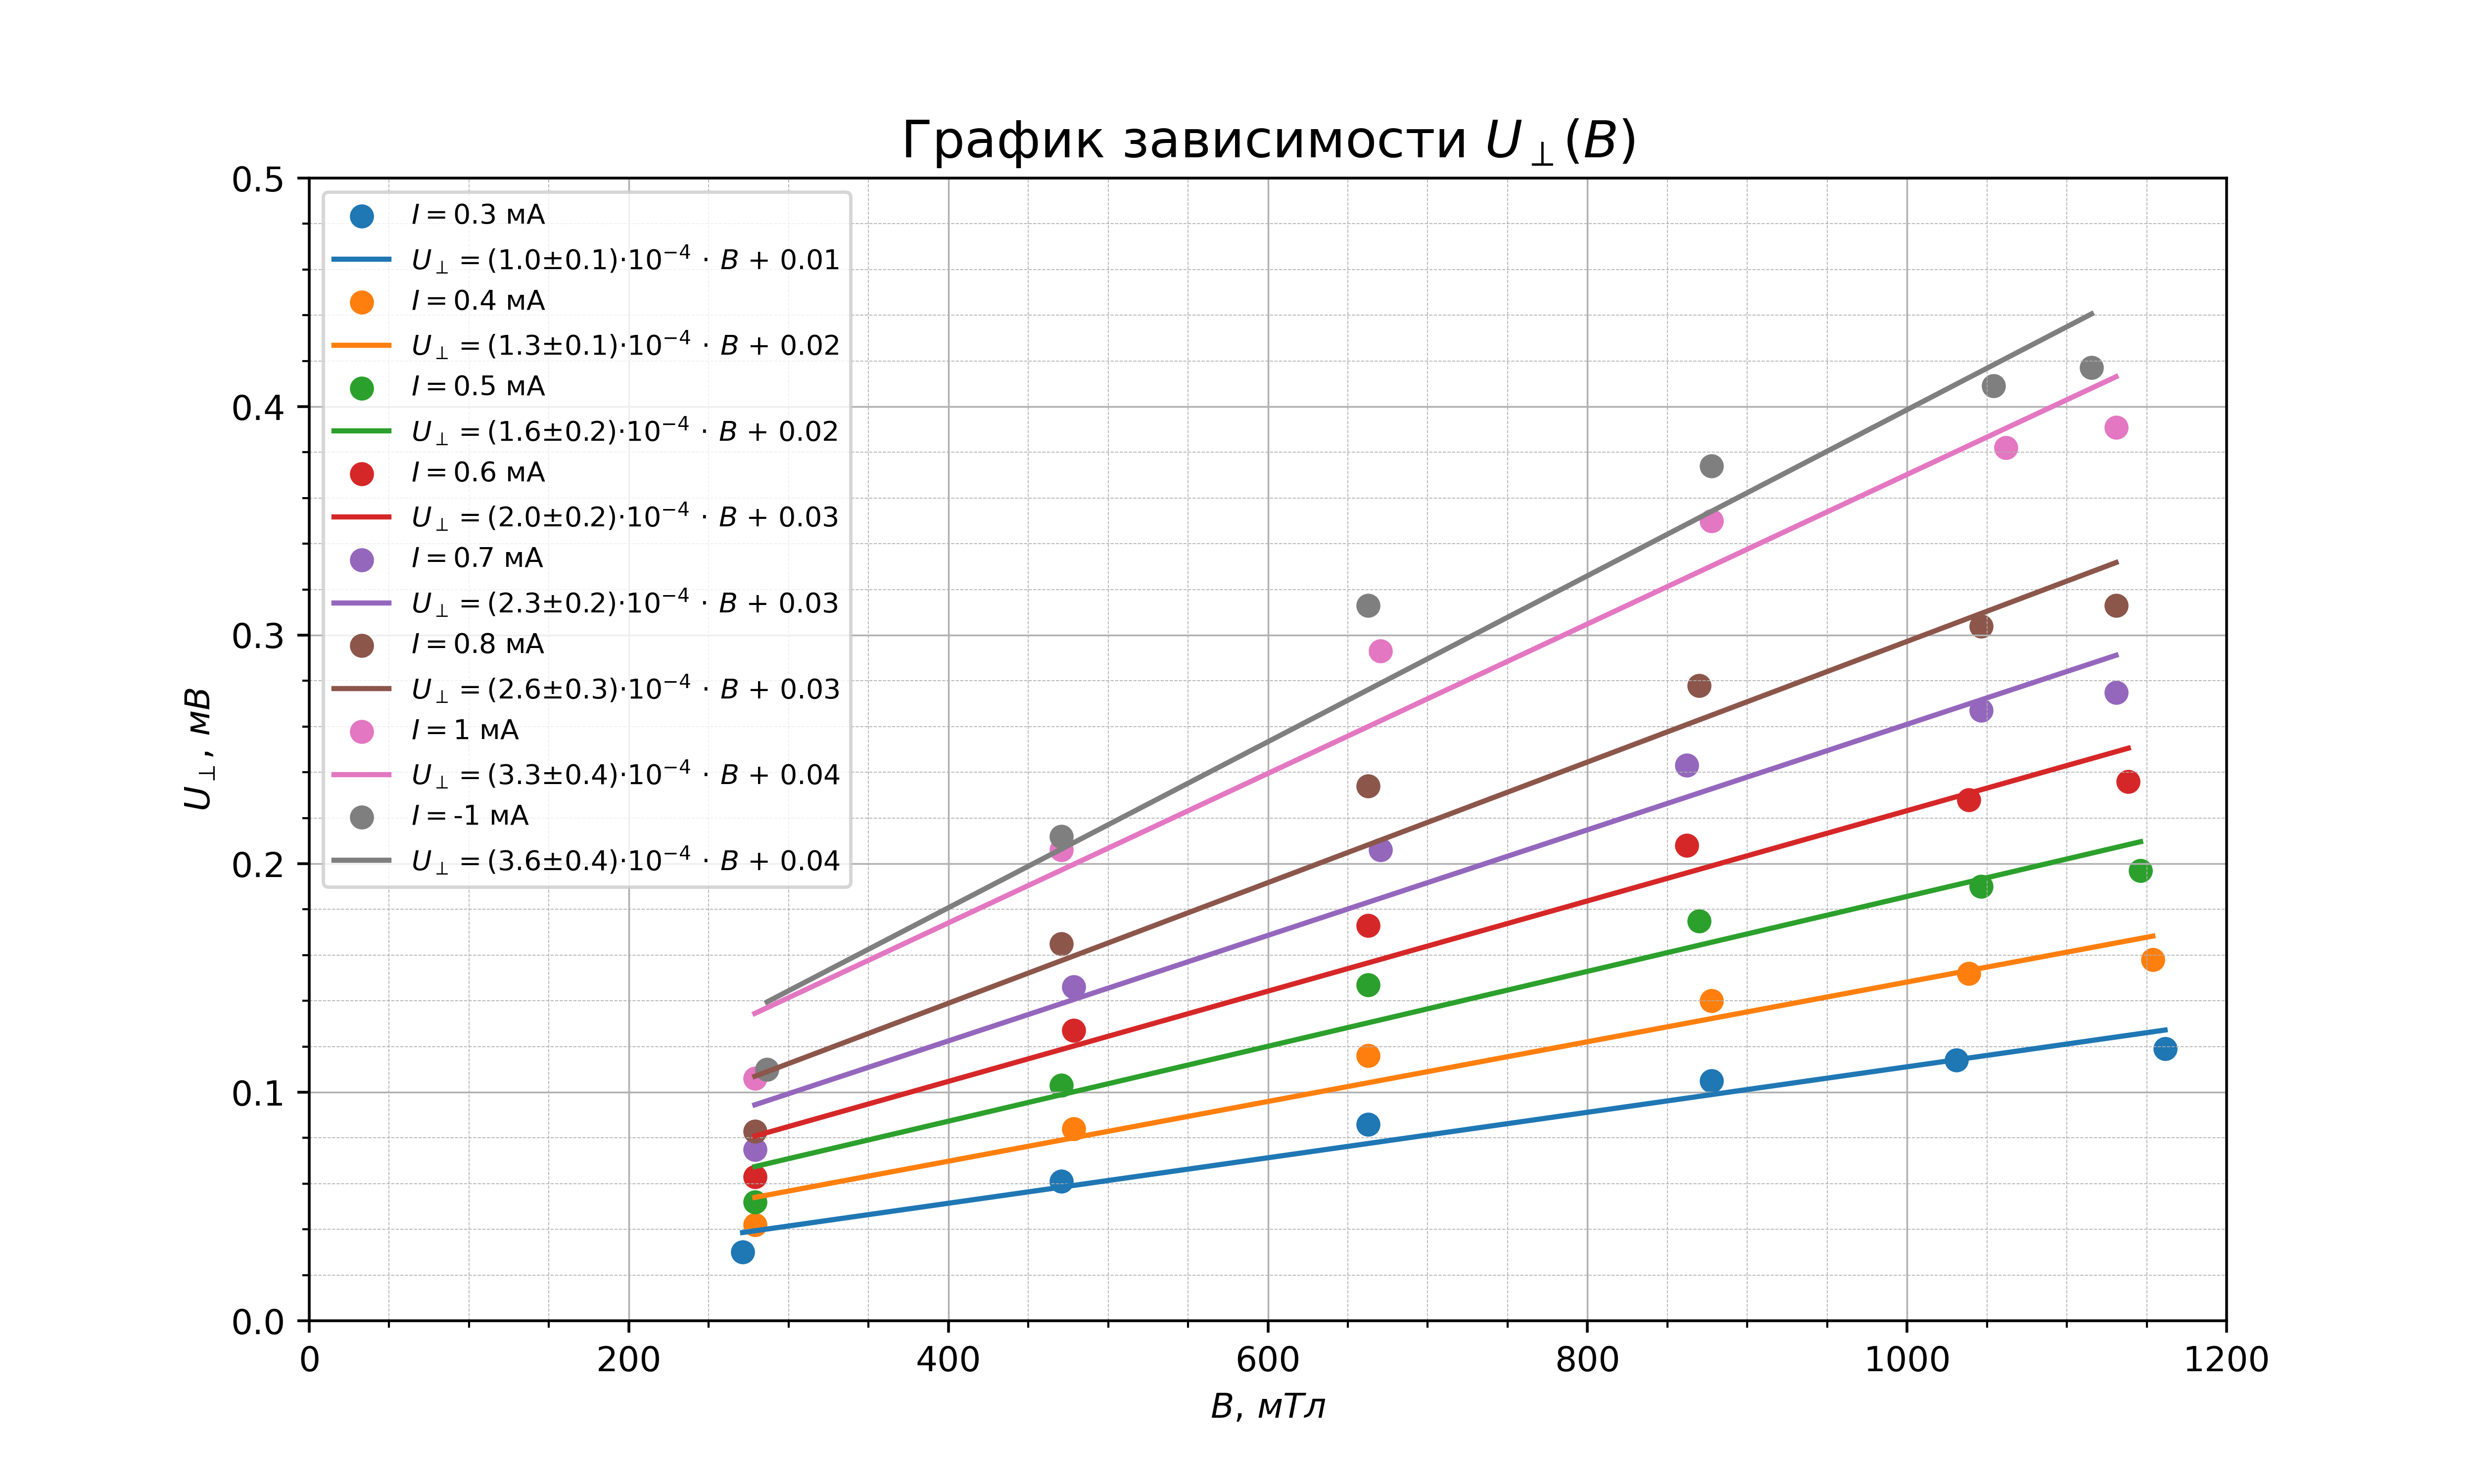
\includegraphics[scale=0.7]{3.3.4_2.png}
\end{center}
\caption{График зависимостей $U_{\perp}(B)$}
\label{plot2}
\end{figure}

\newpage

Знак потенциала соответствует заряду на 3 контакте, значит на нём будут скапливаться дырки. Исходя из геометрии образца, изображённой на рис.~\ref{ris3}, получаем, что основными носителями заряда являются дырки, т. е. имеет место дырочная проводимость.

\begin{figure}[h!]
\begin{center}
    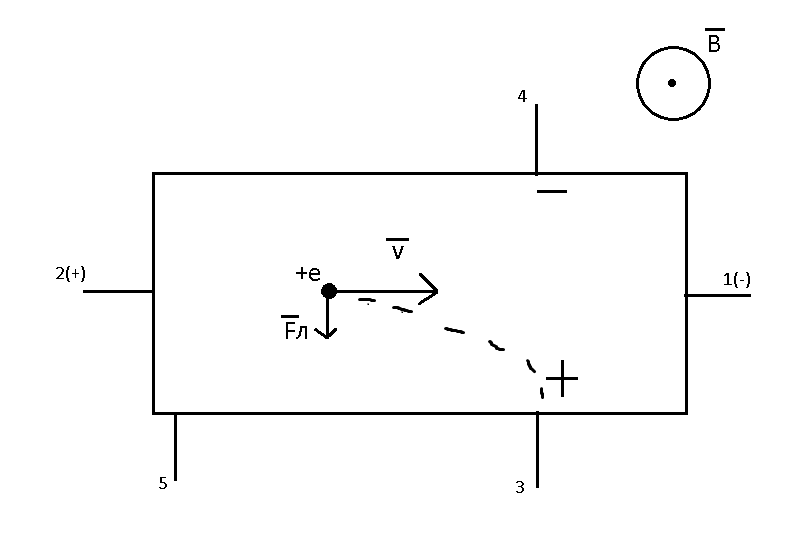
\includegraphics[scale=0.5]{pic.png}
\end{center}
\caption{Направление тока, вектора магнитного поля и отклонение носителей}
\label{ris3}
\end{figure}

\newpage

График зависимости $k = \frac{dU_{\perp}}{dB}$ от тока $I$ представлен на рис.~\ref{plot3}.

\begin{figure}[h!]
\begin{center}
    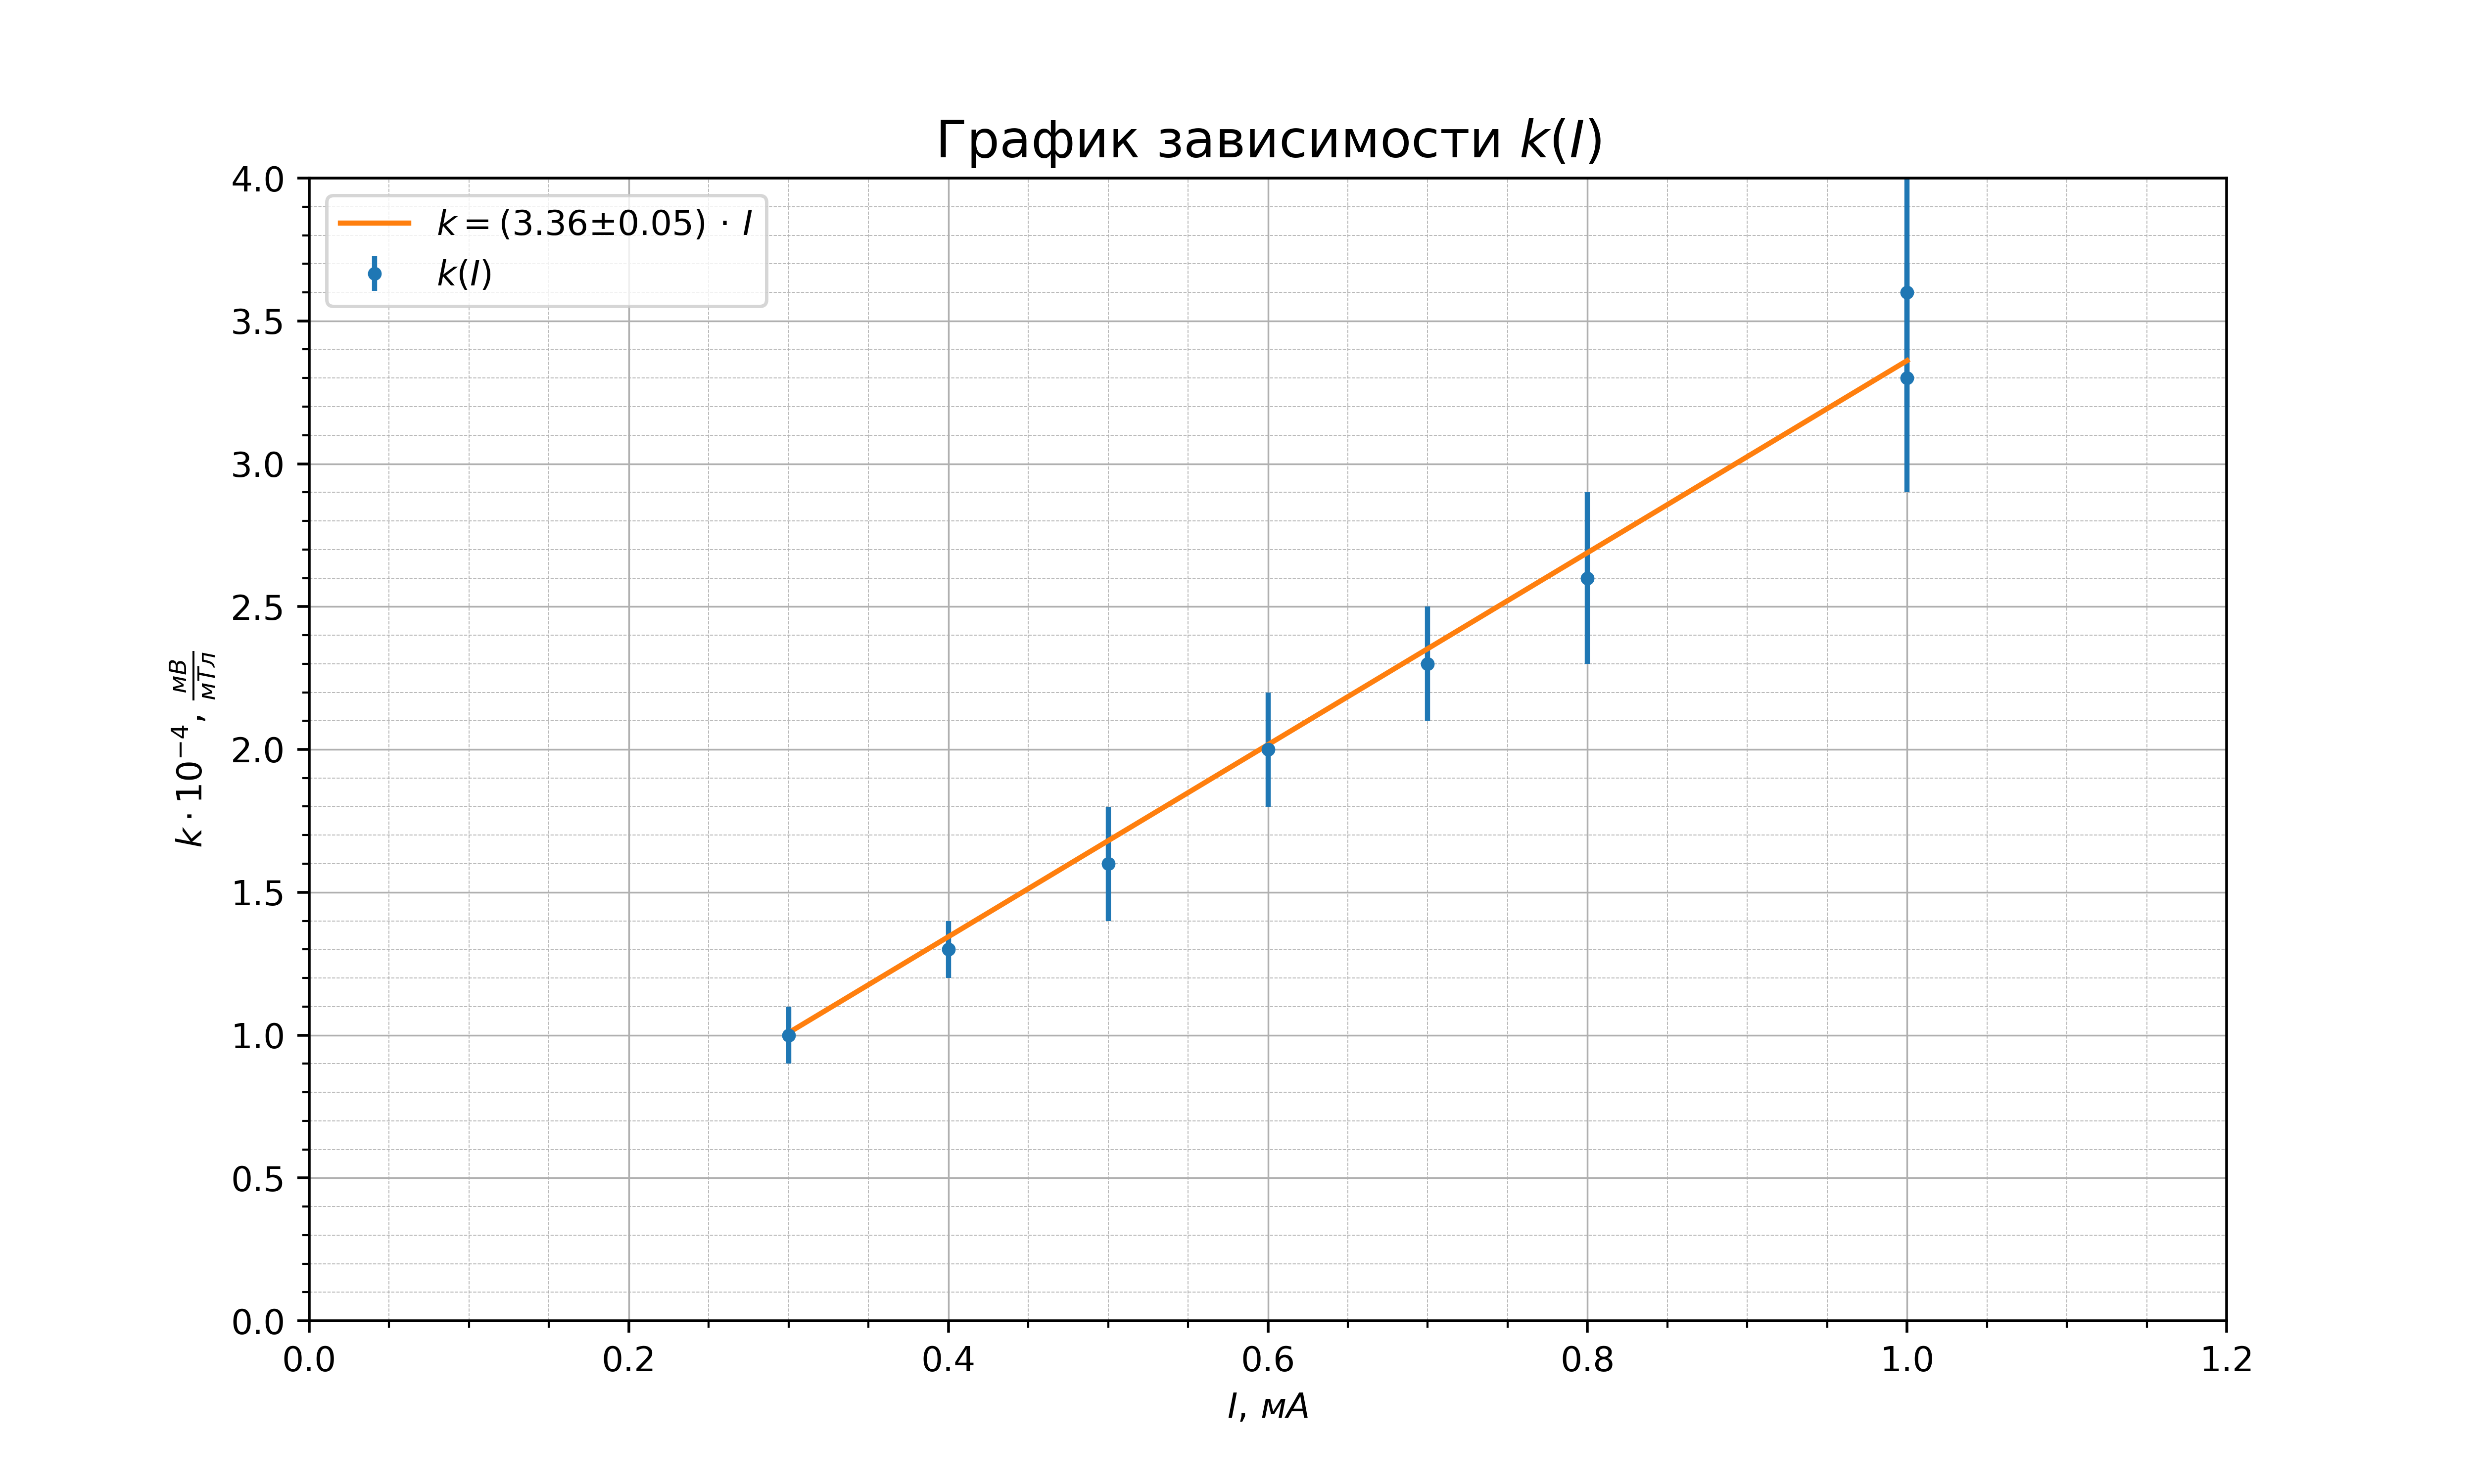
\includegraphics[scale=0.6]{3.3.4_3.png}
\end{center}
\caption{График зависимости $k(I)$}
\label{plot3}
\end{figure}

Получаем угловой коэффициент $\alpha = 0,336\pm0,005~\frac{B}{A \cdot Тл}$. Тогда постоянная Холла \newline $R_H = \alpha \cdot h = (739\pm35) \cdot 10^{-6}~\frac{м^3}{Кл}$.

Рассчитаем концентрацию носителей заряда по формуле $n = \frac{1}{R_H q} = (8,5\pm0,2) \cdot 10^{21}~\frac{1}{м^3}$.

При токе $I = 1~мА$ разность потенциалов между контактами 3 и 5 \newline $U_{35} = -1,980\pm0,001~В$. Вычислим удельную проводимость по формуле \eqref{sigma}: \newline $\sigma_0 = 196,7\pm16,1~{Ом \cdot м}^{-1}$. Тогда удельное сопротивление $\rho_0 = 1/\sigma_0 = 0,0050\pm0,0004~{Ом \cdot м}$.

Подвижность носителей заряда рассчитывается по формуле $\mu = \frac{\sigma}{e n} = 1446\pm123~\frac{см^2}{В \cdot с}$.

\section{Обсуждение результатов и выводы}

В данной работе была исследована зависимость ЭДС Холла от величины магнитного поля при различных значениях тока через образец. Были определены постоянная Холла, подвижность и концентрация носителей заряда в образце легированного германия. Полученные значения:
$$\boxed{R_H = (739\pm35) \cdot 10^{-6}~\frac{м^3}{Кл}, \quad n = (8,5\pm0,2) \cdot 10^{21}~\frac{1}{м^3}, \quad \mu = 1446\pm123~\frac{см^2}{В \cdot с}}$$

Табличное значение собственной концентрации носителей зарядов для германия $n_0 = 2,4 \cdot 10^{13}~\frac{1}{м^3}$. Это меньше полученного значения, что говорит о том, что данный образец германия содержит примеси. Основной вклад в погрешность вносит погрешность определения коэффициентов зависимости. Также на ошибку измерений может влиять зависимость концентрации основных носителей заряда от температуры, ярко выраженная в полупроводниках.

\end{document}
